%! TEX program = LuaTeX

\documentclass[nobackground,dvipsnames,table,aspectratio=169]{beamer}
\usepackage{cs152}

\mode<presentation>
{\usetheme{Hannover}
    \usecolortheme{cs152}
    \setbeamercovered{transparent}
    \useinnertheme[shadow=false]{rounded}
    \usebackgroundtemplate{}
    \setbeamercolor*{frametitle}{parent=palette primary}
    \setbeamerfont{block title}{size={}}
    \setbeamertemplate{navigation symbols}{}
}

\title{Dating Apps and the Sharing Economy}
\subtitle{CS 152 --- Lecture 13}

\author[A. Stamos]{Alex Stamos}
\institute[Stanford University]{Stanford Cyber Policy Center}
\date[2022]{\today}
\subject{CS 152 --- Trust and Safety Engineering}
%\titlegraphic{
\includegraphics[width=5cm]{img/cyber-logo-white-black-red-WEB}}

% Change the level of bulleting on the ToC page
\setcounter{tocdepth}{2}

\graphicspath{{img/lesson13}}

\begin{document}

\begin{frame}
    \titlepage
\end{frame}

\begin{frame}{}
    \thispagestyle{empty}
    \AddToShipoutPictureBG*{
\includegraphics[width=\paperwidth]{content-warning}}
\end{frame}

\begin{frame}{Jane Doe}
    \centering
    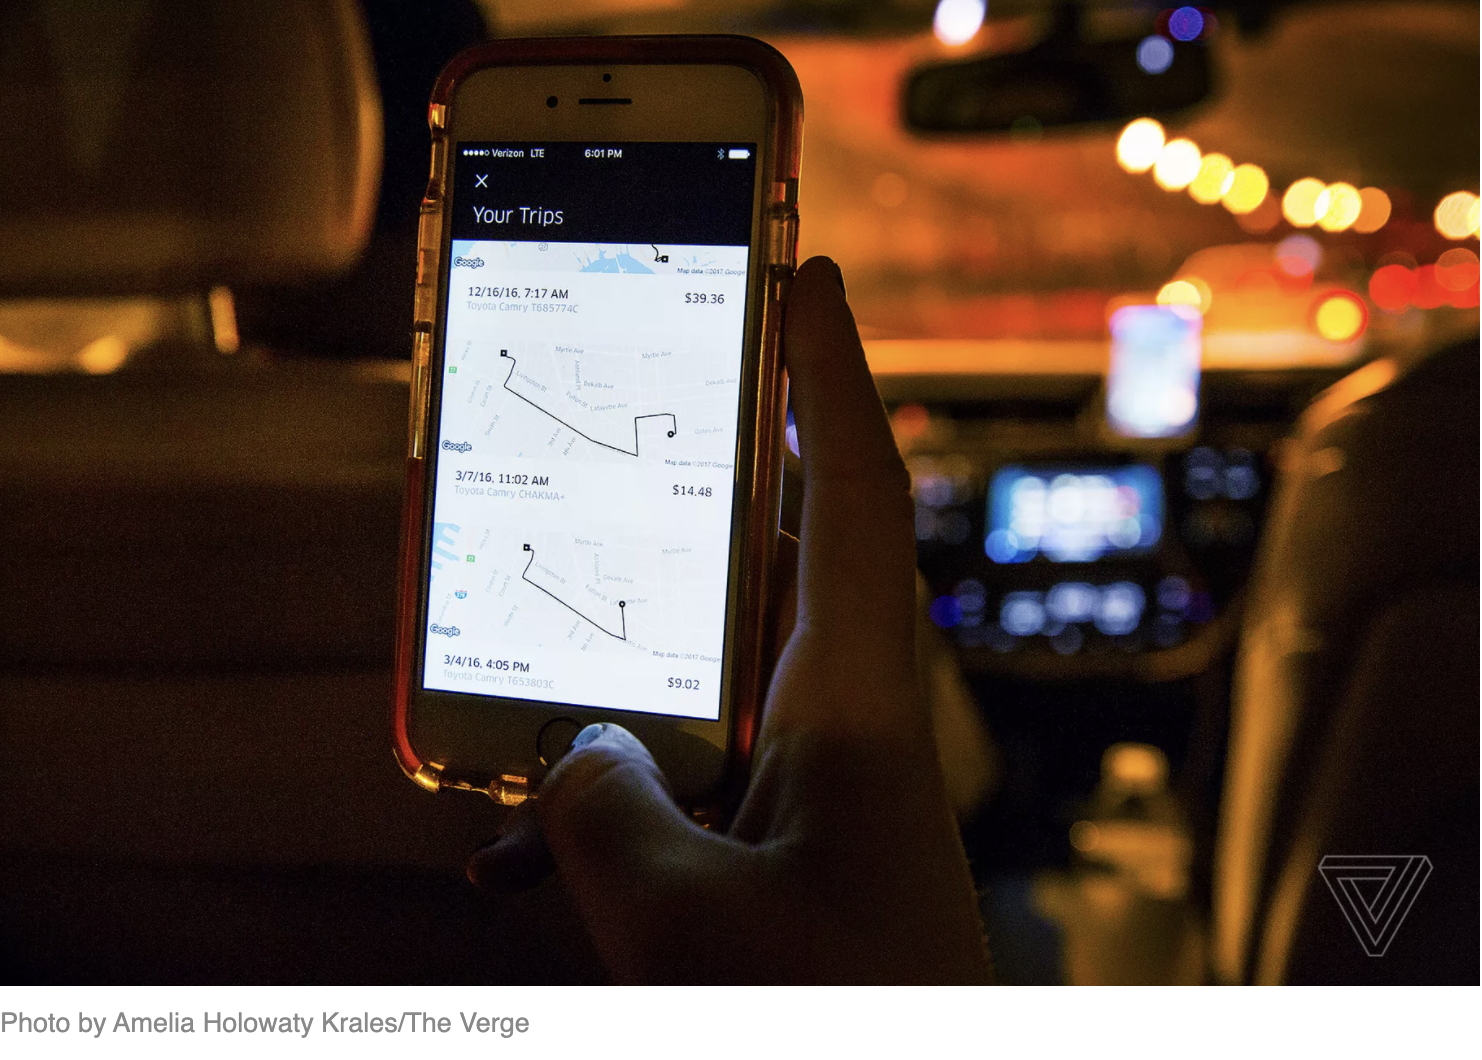
\includegraphics[height=0.85\textheight]{jane-doe}
\end{frame}

\begin{frame}{Safest Ride on the Road?}
    \centering
    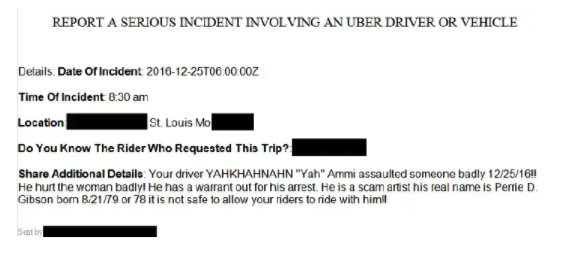
\includegraphics[width=0.6\textwidth]{uber-report-driver-1}
    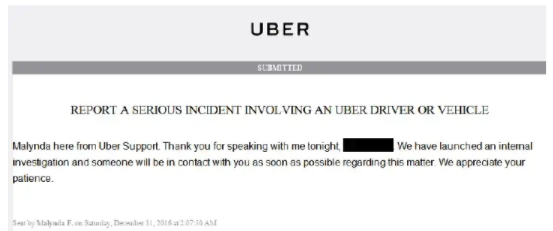
\includegraphics[width=0.6\textwidth]{uber-report-driver-2}
\end{frame}

\begin{frame}{Difference Between Policies and Implementation}
    \centering
    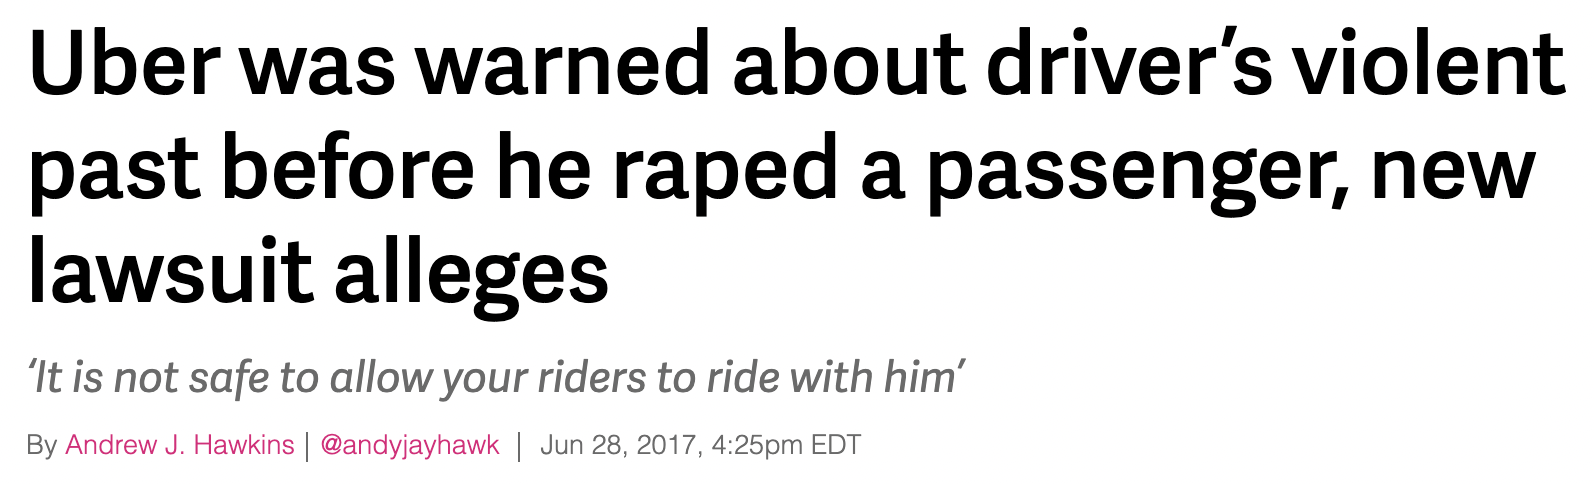
\includegraphics[width=\textwidth]{uber-reported-driver-headline}
\end{frame}

\section{IRL Platforms}

\begin{frame}{"In Real Life" (IRL) Platforms}
    \begin{itemize}
        \item \textbf{New class of issues} for products that put humans together-usually strangers-for some kind of interaction that used to be much higher friction
        \item \textbf{Creates a number of new risks} related to those we’ve discussed, but that can be higher stakes because of the physical interactions they entail
        \item \textbf{Many safety issues IRL platforms face involve breaking laws in the real world} (burglery, rape, murder), use of Section 230 is controversial
        \item Safety of users is dependent on \textbf{design choices of platforms}
    \end{itemize}
\end{frame}

\begin{frame}{What Are You Disrupting?}
    \begin{columns}
        \column{0.4\textwidth}
            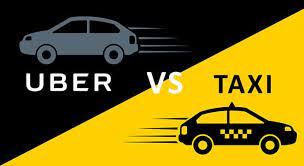
\includegraphics[width=\textwidth]{uber-vs-taxi}
            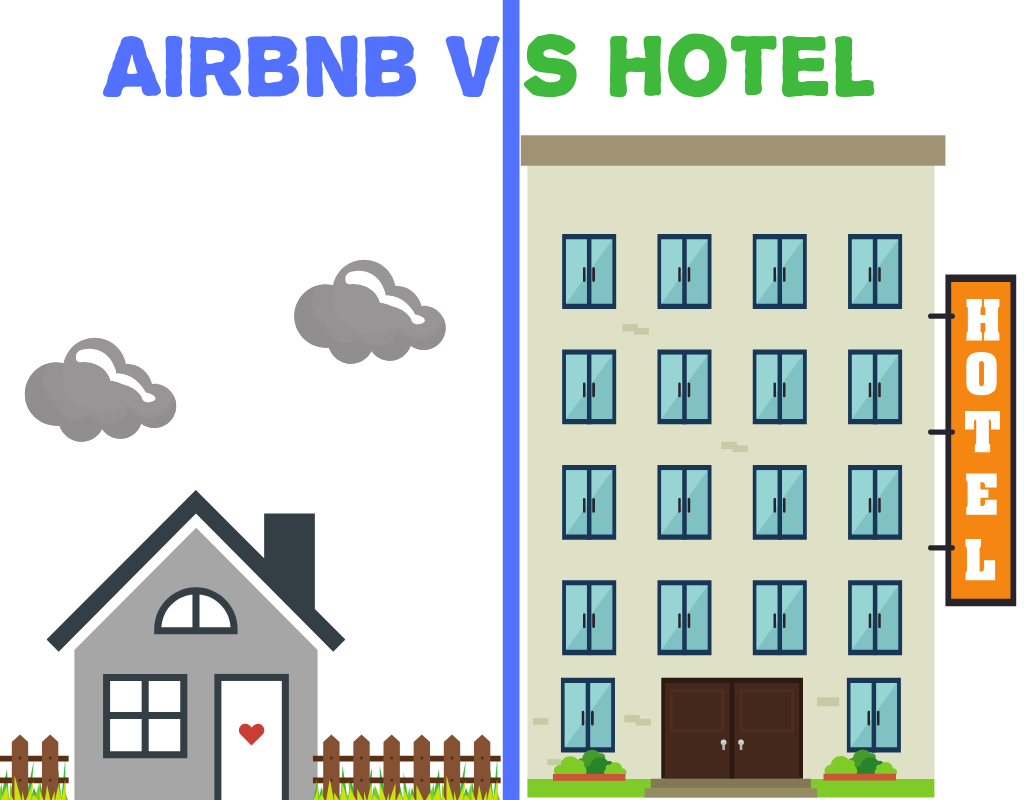
\includegraphics[width=\textwidth]{airbnb-vs-hotel}
        \column{0.6\textwidth}
            \begin{itemize}
                \item IRL platforms often \textbf{intend to disrupt} existing industries.
                \item Can’t just understand downstream economic effects.
                \item Also need to think about safety challenges these industries face that you could exacerbate.
                \item Can be an opportunity to \textbf{make things better.}
            \end{itemize}
    \end{columns}
\end{frame}

\begin{frame}{Disrupted Industries: Uber vs. Taxi}
    \begin{columns}
        \column{0.5\textwidth}
            \centering
            \textbf{Uber}\\~\\
            Outsources background checks to third party services\\~\\
            Public safety reports (6,000 reported sexual assaults in Uber between 2017-2018)\\~\\
            Drivers are independent contractors\\~\\
            Uber removed a driver from accessing the app while an assault investigation is underway\\~\\
        \column{0.5\textwidth}
            \centering
            \textbf{Taxi}\\~\\
            Conducts background checks using fingerprint database run by FBI\\~\\
            No public released assault statistics, public reports are likely inaccurate (San Francisco taxi users reported 14 incidents of “violence or physical altercations” in 2017)\\~\\
            Drivers are employees\\~\\
            Drivers are suspended when criminal charges are filed\\~\\
    \end{columns}
\end{frame}

\begin{frame}{Opposing Equities in Policies}
    \begin{columns}
        \column{0.4\textwidth}
            \adjincludegraphics[trim=0 60 0 60, clip, width=\textwidth]{airbnb}
            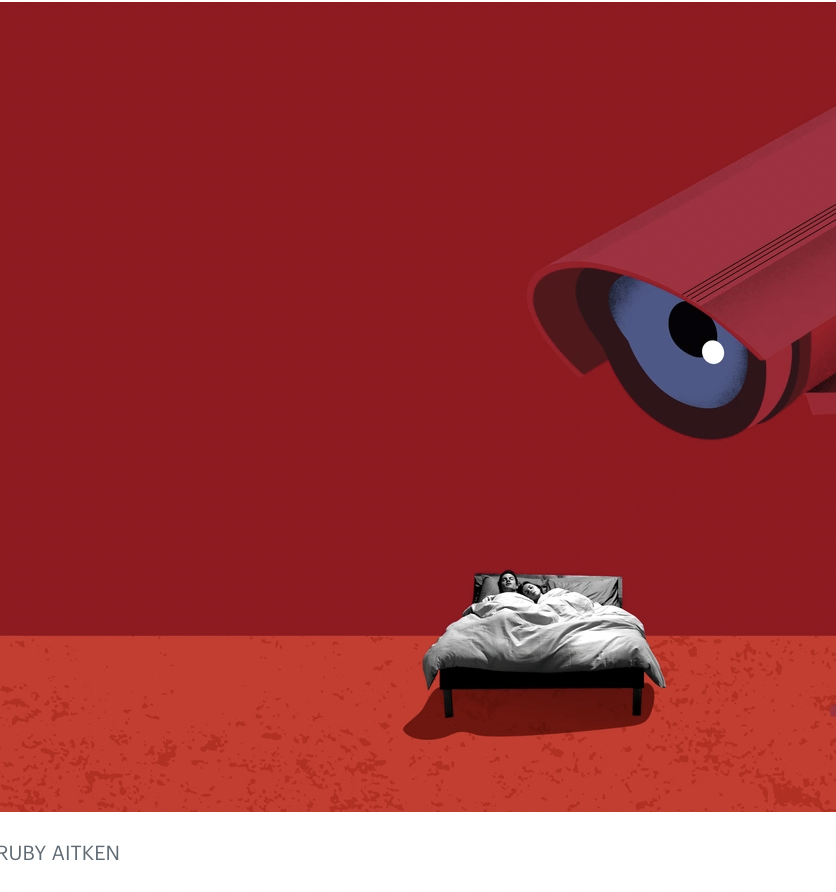
\includegraphics[width=\textwidth]{airbnb-surveillance}
        \column{0.6\textwidth}
            \begin{itemize}
                \item \textbf{Hosts} have reasons they may want security cameras (safety, stealing etc.)
                \item \textbf{Guests} have reasons they don’t want to be filmed, especially in private spaces
            \end{itemize}
    \end{columns}
\end{frame}

\section{Marketplaces}

\begin{frame}{What Is This?}
    \centering
    \adjincludegraphics[trim=40 0 120 240, clip, width=0.9\textwidth]{first-item-sold-on-ebay}
\end{frame}

\begin{frame}{Commerce / Social}
    \begin{columns}
        \centering
        \column{0.5\textwidth}
            \centering
            \begin{columns}
                \column{0.5\textwidth}
                    \centering
                    
\includegraphics[width=0.8\textwidth]{ebay}
                \column{0.5\textwidth}
                    \centering
                    
\includegraphics[width=0.8\textwidth]{etsy}
            \end{columns}
            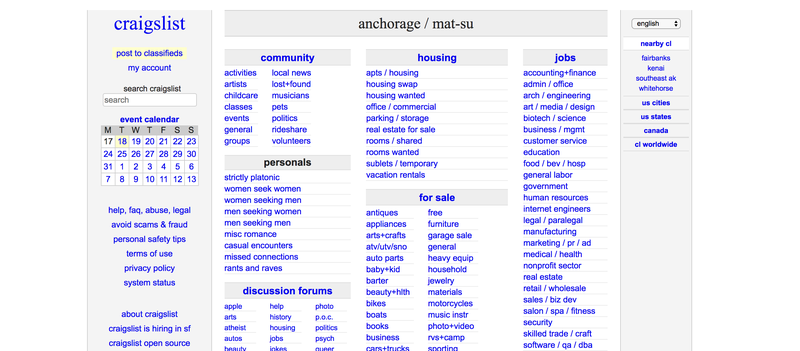
\includegraphics[width=\textwidth]{craigslist}
        \column{0.5\textwidth}
            \begin{itemize}
                \item Suddenly everyone can be a retailer!
                \item Early days, put cash in an envelope and pray
                \item Inevitable fraud: fake items/rip-offs
            \end{itemize}
    \end{columns}
\end{frame}

\begin{frame}{Facebook Marketplace: Human Trafficking}
    \centering
    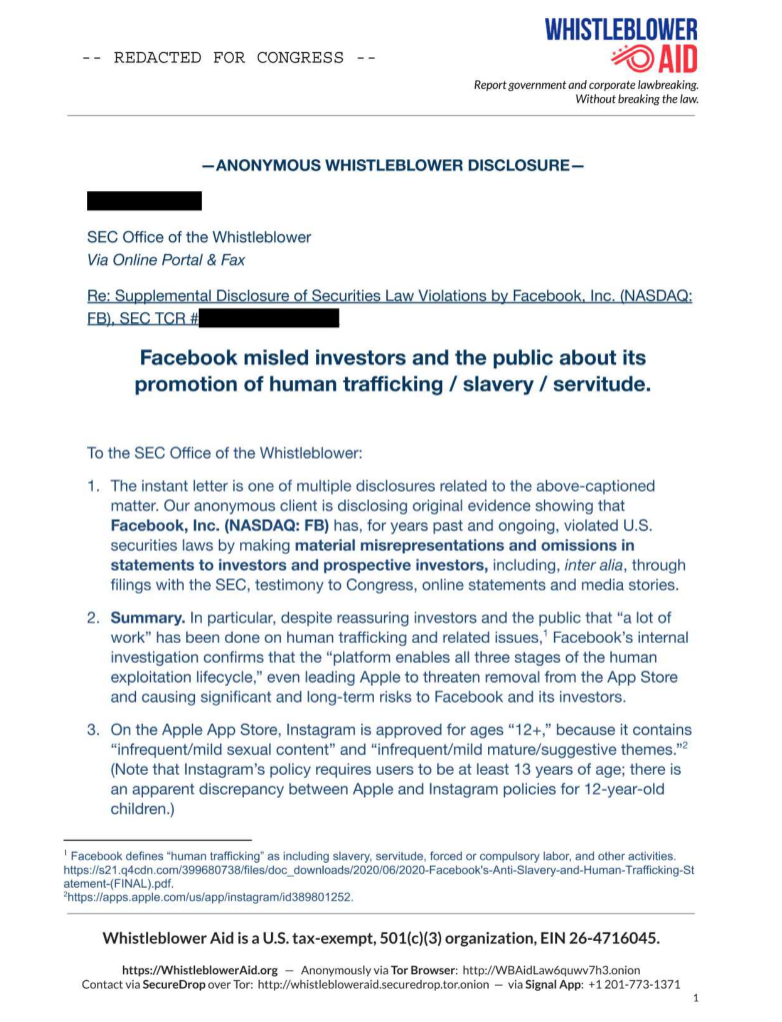
\includegraphics[height=0.85\textheight]{facebook-human-trafficking-whistleblower}
\end{frame}

\section{Dating Apps}

\begin{frame}{Dating Apps: White Lies to Serious Crimes}
    \begin{columns}
        \column{0.5\textwidth}
            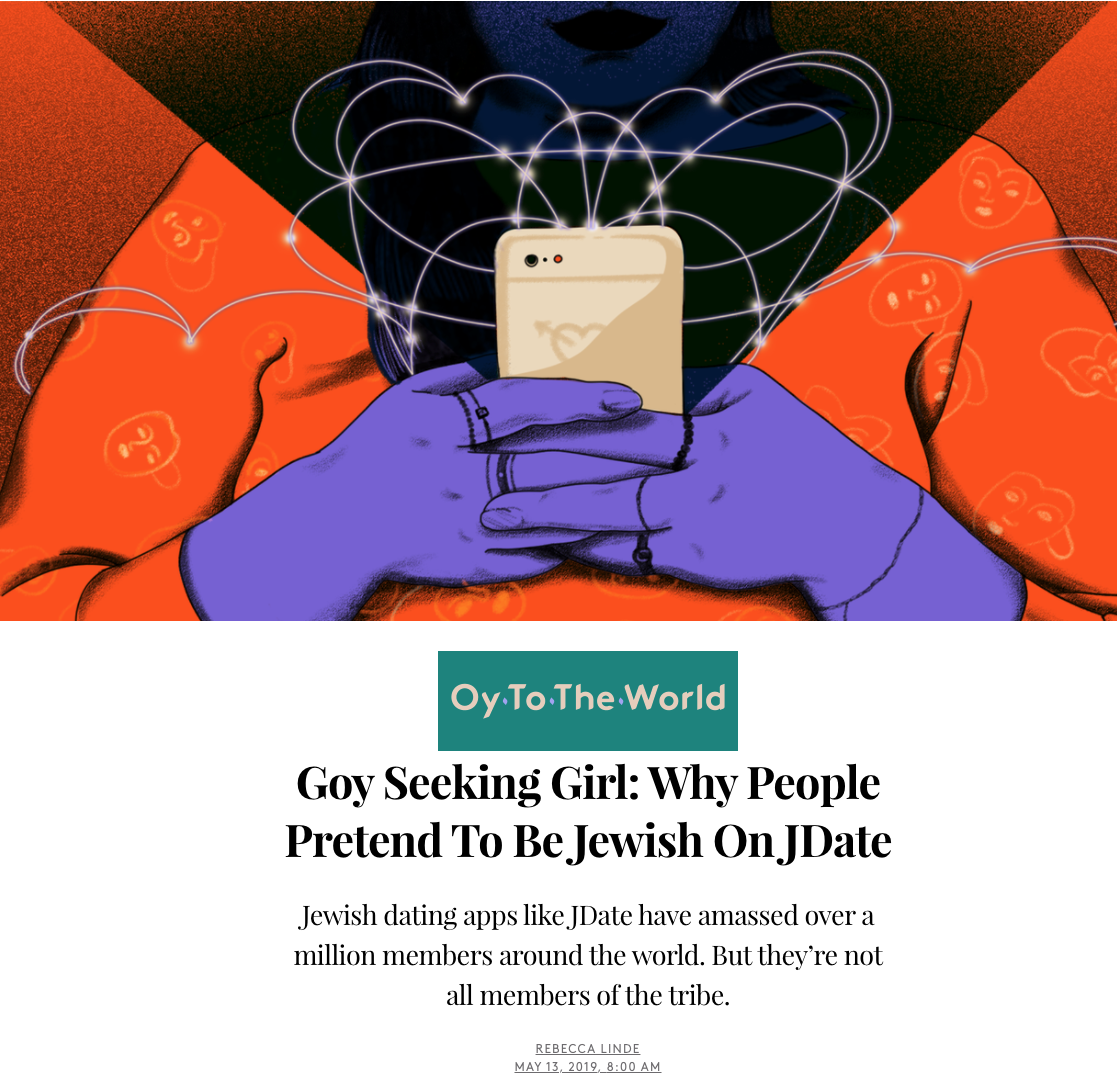
\includegraphics[width=\textwidth]{dating-app-lies}
        \column{0.5\textwidth}
            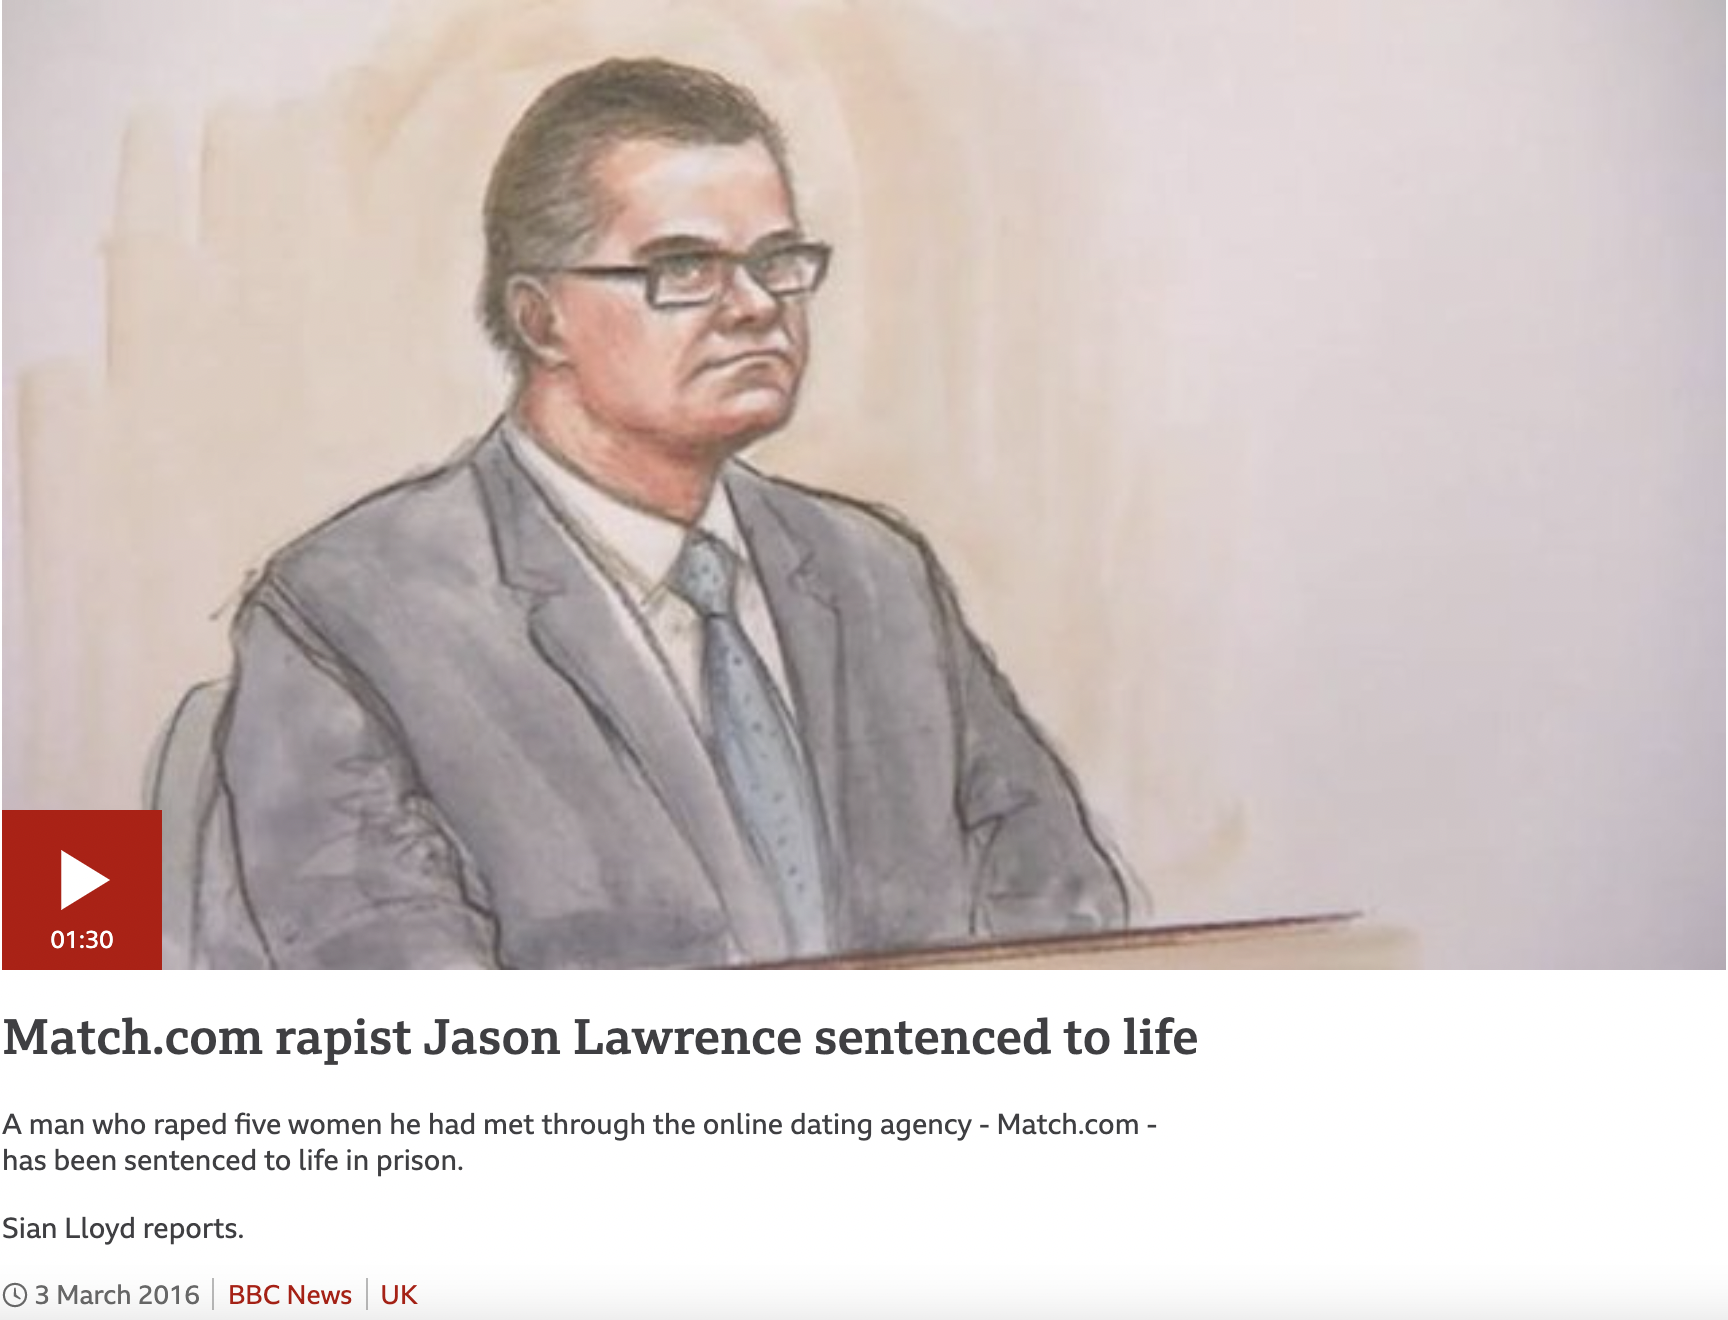
\includegraphics[width=\textwidth]{dating-app-crimes}
    \end{columns}
\end{frame}

\begin{frame}{Dating Apps}
    \begin{columns}
        \column{0.5\textwidth}
            \centering
            \adjincludegraphics[trim= 0 100 0 100, clip, width=\textwidth]{bumble}
            \begin{columns}
                \column{0.5\textwidth}
                    
\includegraphics[width=\textwidth]{jdate}
                \column{0.5\textwidth}
                    
\includegraphics[width=\textwidth]{match}
            \end{columns}
            
\includegraphics[trim= 60 100 40 100, clip, width=\textwidth]{grindr}
        \column{0.5\textwidth}
            \begin{itemize}
                \item Use of online dating apps has skyrocketed
                \item Dating apps face a number of challenges from age verification to honey trapping, to targeted killings, to global surveillance 
                \item Risks have created a marketplace for apps with stronger identity and T\&S policies
            \end{itemize}
    \end{columns}
\end{frame}

\begin{frame}{Geolocation is a Common Safety/Privacy Problem}
    \begin{columns}
        \column{0.5\textwidth}
            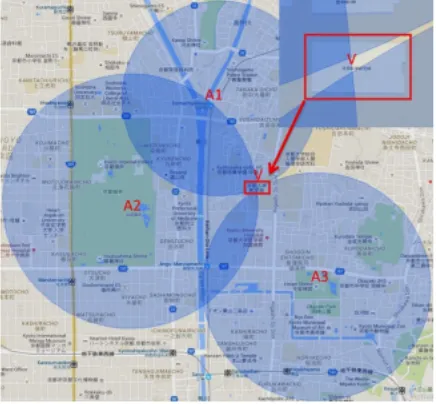
\includegraphics[width=\textwidth]{trilateration}
            \scriptsize
            A MAP SHOWING A BASIC TRILATERATION ATTACK, IN WHICH LEARNING THE DISTANCE FROM THREE POINTS TO A TARGET ALLOWS THE VICTIM "V" TO BE PINPOINTED.
        \column{0.5\textwidth}
            \begin{itemize}
                \item Grindr willingly shares high-accuracy location data
                \item Meant to have an option to disable location-sharing, but was only surface-level
                \item \textbf{Trilateration:} Can determine the exact location by combining the distance measurement from 3 points surrounding
            \end{itemize}
    \end{columns}
\end{frame}

\begin{frame}{Grindr and Global Persecution and Surveillance}
    \begin{columns}
        \column{0.4\textwidth}
            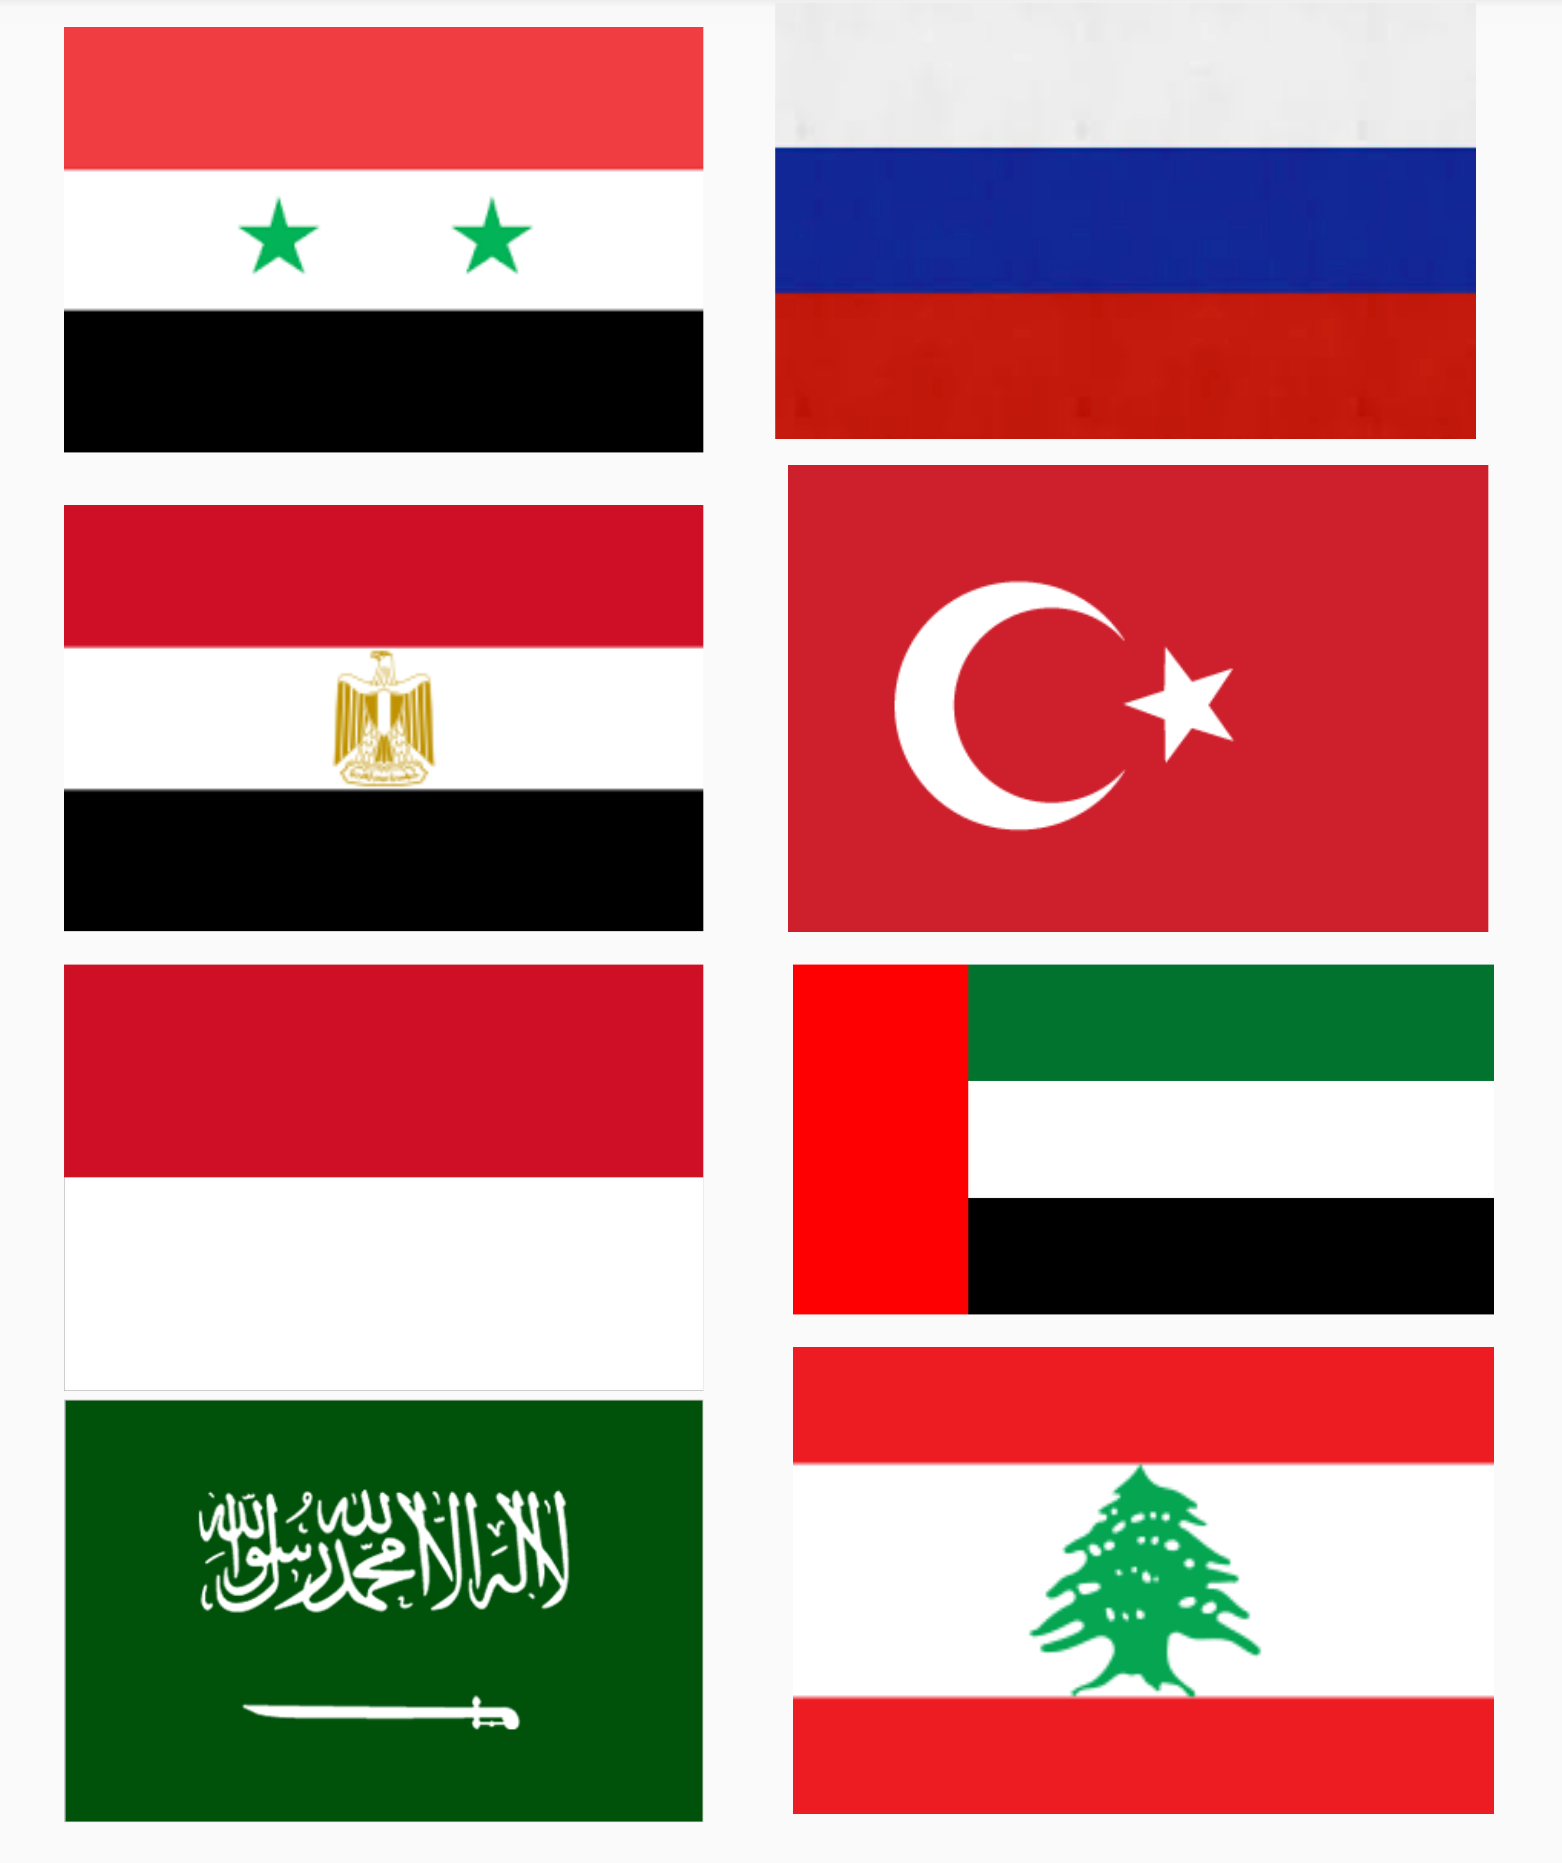
\includegraphics[width=\textwidth]{flags}
        \column{0.6\textwidth}
            \begin{itemize}
                \item Syrian gay men lured into "dates" by members of ISIS, and then arrested and stoned to death. 
                \item In Russia, gay men have been trapped and beaten by thugs in countless incidents.
                \item Egyptian police have used dating apps such as Grindr to track and arrest Gay people.
                \item Grindr partially or entirely blocked in Turkey, Saudi Arabia, the United Arab Emirates, Indonesia, and Lebanon.
            \end{itemize}
    \end{columns}
\end{frame}

\begin{frame}{\textbf{Exercise:} What Could Go Wrong? How Could You Mitigate Harm?}
    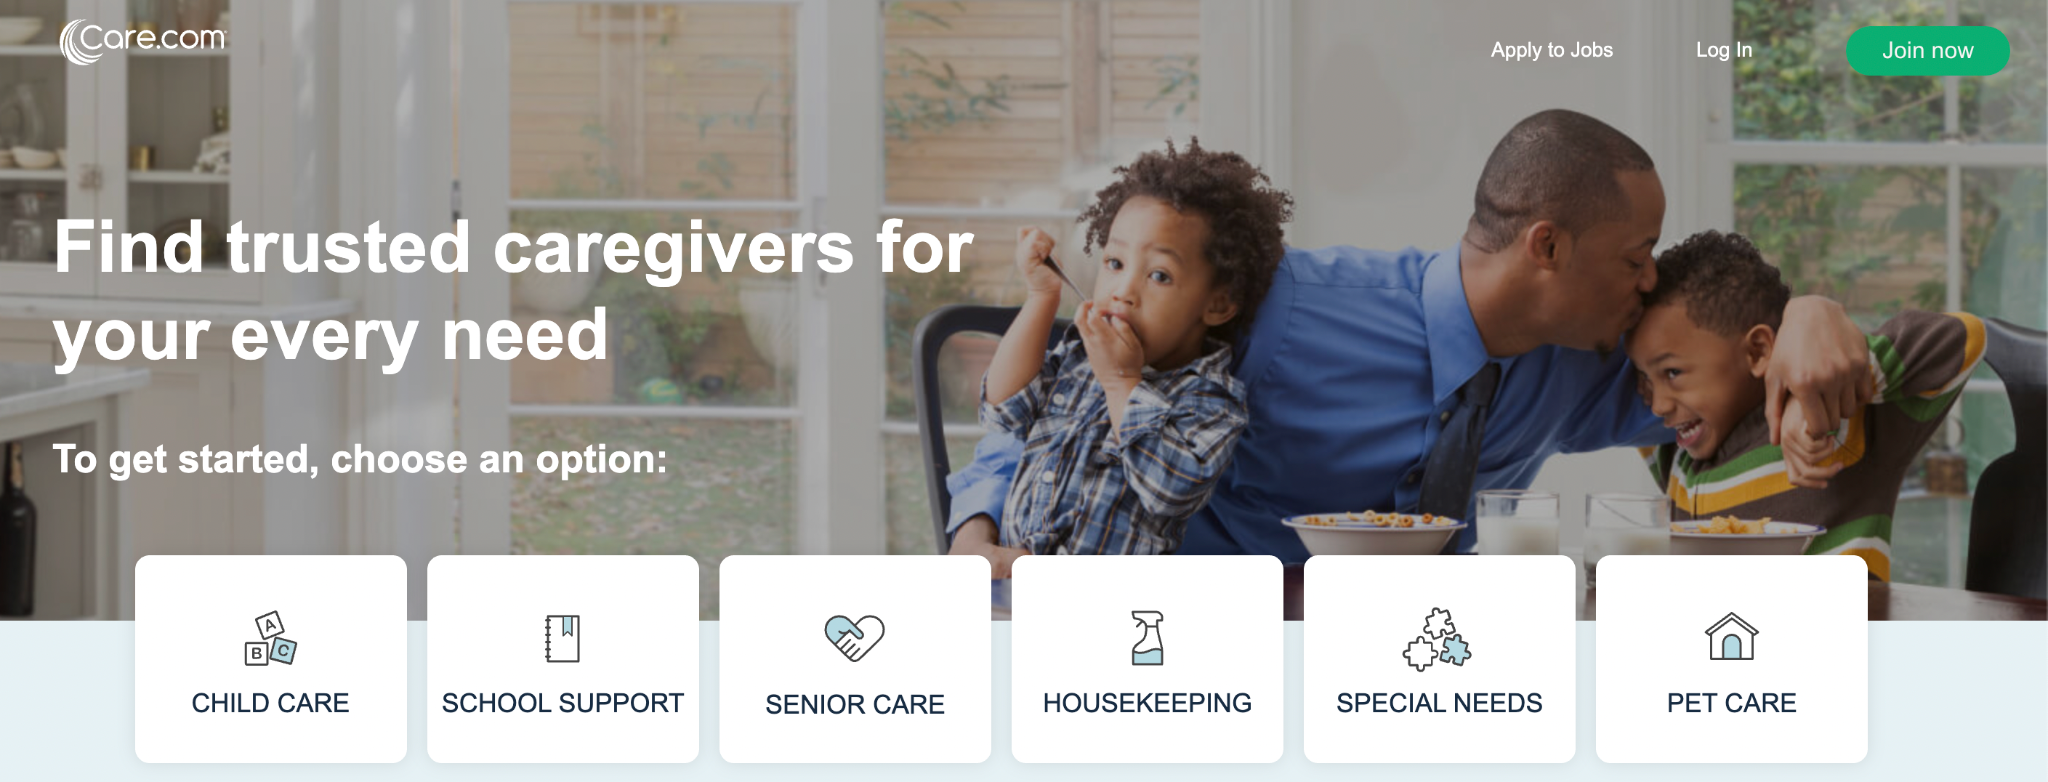
\includegraphics[width=\textwidth]{care-com}
\end{frame}

\section{Responses and Mitigations}

\begin{frame}{Policy Responses}
    \large
    \begin{itemize}
        \item Set rules for interactions above the law (not necessarily illegal, but maintain brand trust and values)
        \item Enforce identity (Background checks, validation etc.)
        \item Provide 2-way rating systems
        \item Build policy teams
        \item Build investigation teams that can quickly engage with safety issues
        \item Work with local people \& law enforcement in every location where you will operate
        \item Publish measurement and transparency reports
        \item Educate users and employees on risks and mitigations
    \end{itemize}
\end{frame}

\begin{frame}{Brazil Backfire: Including Cash Options to Be Inclusive}
    \begin{columns}
        \column{0.4\textwidth}
            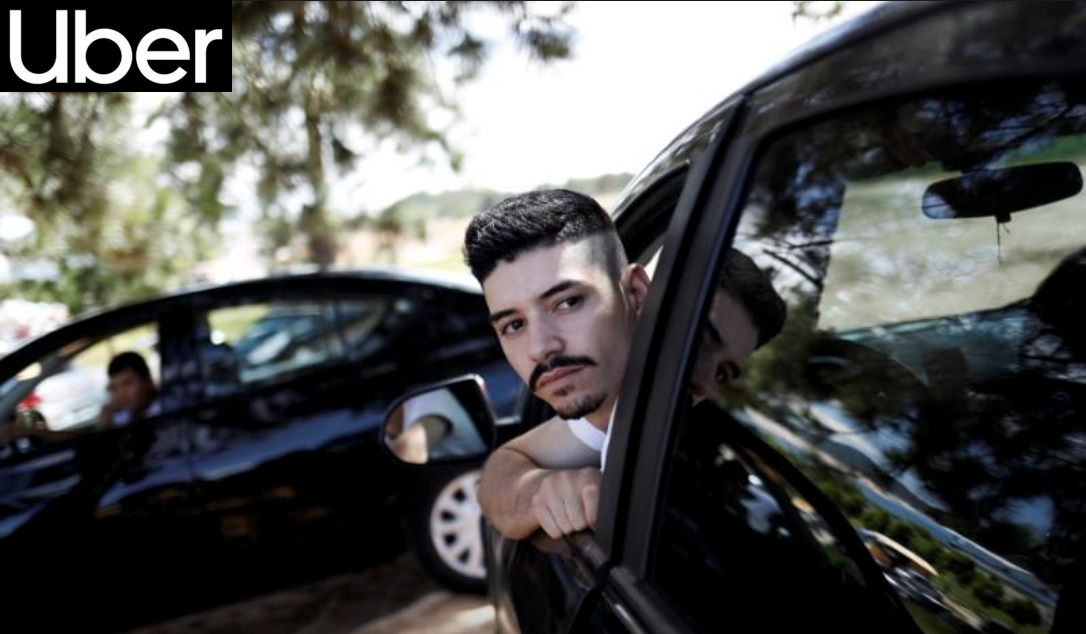
\includegraphics[width=\textwidth]{brazil-uber-1}
            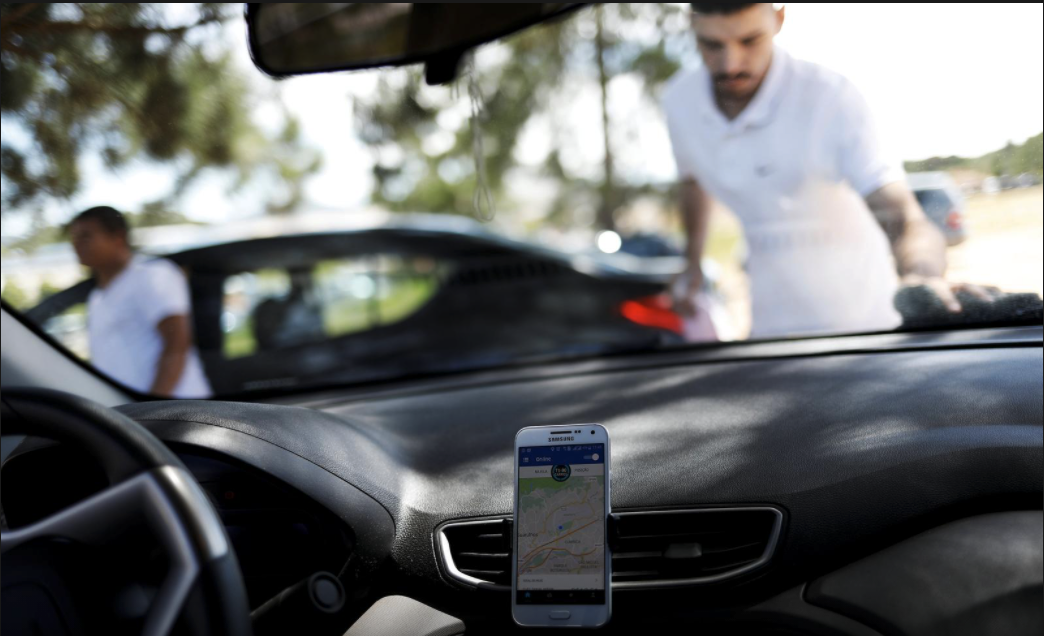
\includegraphics[width=\textwidth]{brazil-uber-2}
        \column{0.6\textwidth}
            \begin{itemize}
                \item Changed the policy in Brazil to grow the new market where many did not have credit cards.
                \item Demand increased (Uber drivers rose ten-fold).
                \item So did crime (avg. 13 attacks pre cash option to 141 per month rest of year post cash option available).
                \item Cash option = easy target for criminals. No credit card to identify them with.
            \end{itemize}
    \end{columns}
\end{frame}

\begin{frame}{Product/Technical Responses}
    \large
    \begin{itemize}
        \item ML on aspects of the listing 
        \item Fake account detection (multiple forms of ID, ties to other social media)
        \item Real differential privacy when needed
        \item 2-way reporting flows
        \item Real-Time GPS
        \item Safety API’s (e.g. Noonlight)
    \end{itemize}
\end{frame}

\begin{frame}{Safety APIs (e.g. Noonlight)}
    \begin{columns}
        \column{0.5\textwidth}
            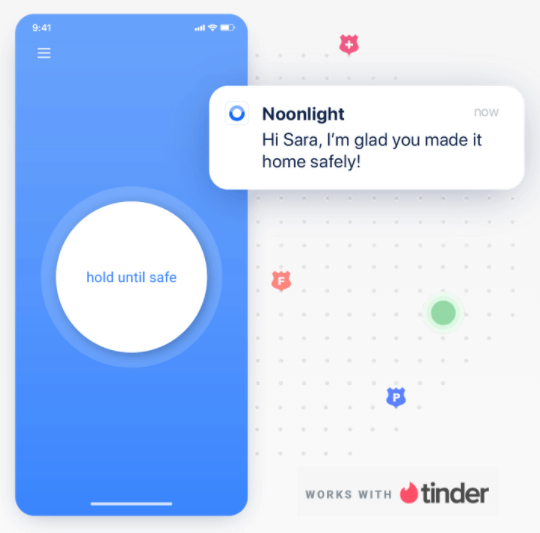
\includegraphics[width=\textwidth]{noonlight}
        \column{0.5\textwidth}
            Suite of emergency response APIs for example:
            \begin{itemize}
                \item Silently summon help to exact location
                \item Save details to a Timeline (who, when, where, meeting)
                \item Data routing to 911 dispatchers and first responders when needed
            \end{itemize}
    \end{columns}
\end{frame}

\begin{frame}{Emergency Buttons}
    \begin{columns}
        \column{0.5\textwidth}
            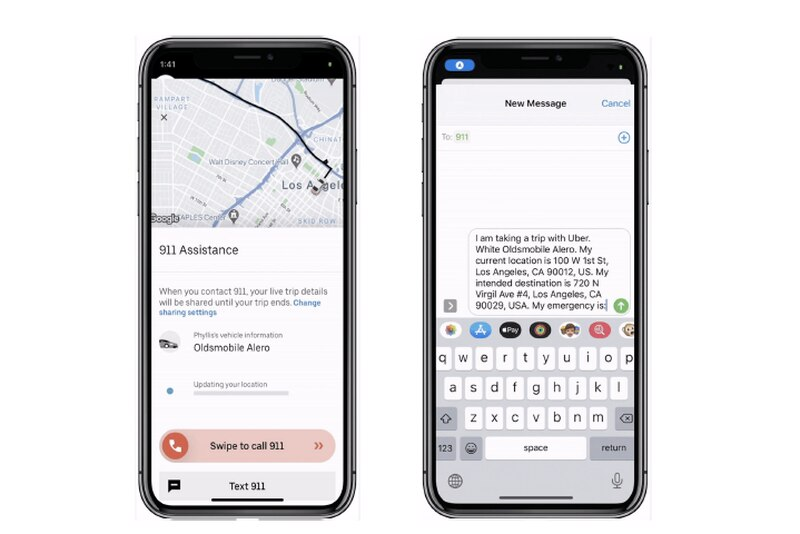
\includegraphics[width=\textwidth]{emergency-buttons}
        \column{0.5\textwidth}
            \begin{itemize}
                \item Initially sent alert to Uber
                \item Then initiated a 911 call
                \item Now allows a text to 911
            \end{itemize}
            Why?
    \end{columns}
\end{frame}

\begin{frame}{Thoughtfull Consider Tensions and Tradeoffs}
    \begin{columns}
        \column{0.5\textwidth}
            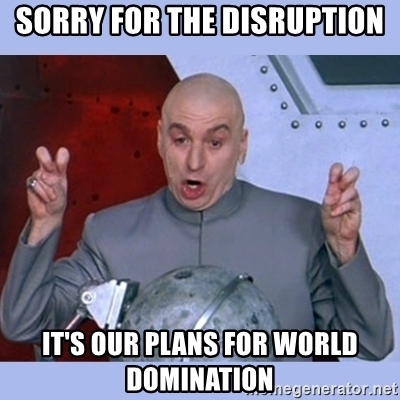
\includegraphics[width=\textwidth]{disruption}
        \column{0.5\textwidth}
            \begin{itemize}
                \item Can’t attribute all harms to tech platforms
                \item Don’t want to make it easier to target victims for crimes
                \item Consider tradeoffs
                \item Due diligence
            \end{itemize}
    \end{columns}
\end{frame}

\begin{frame}{Lifecycle of a Company}
    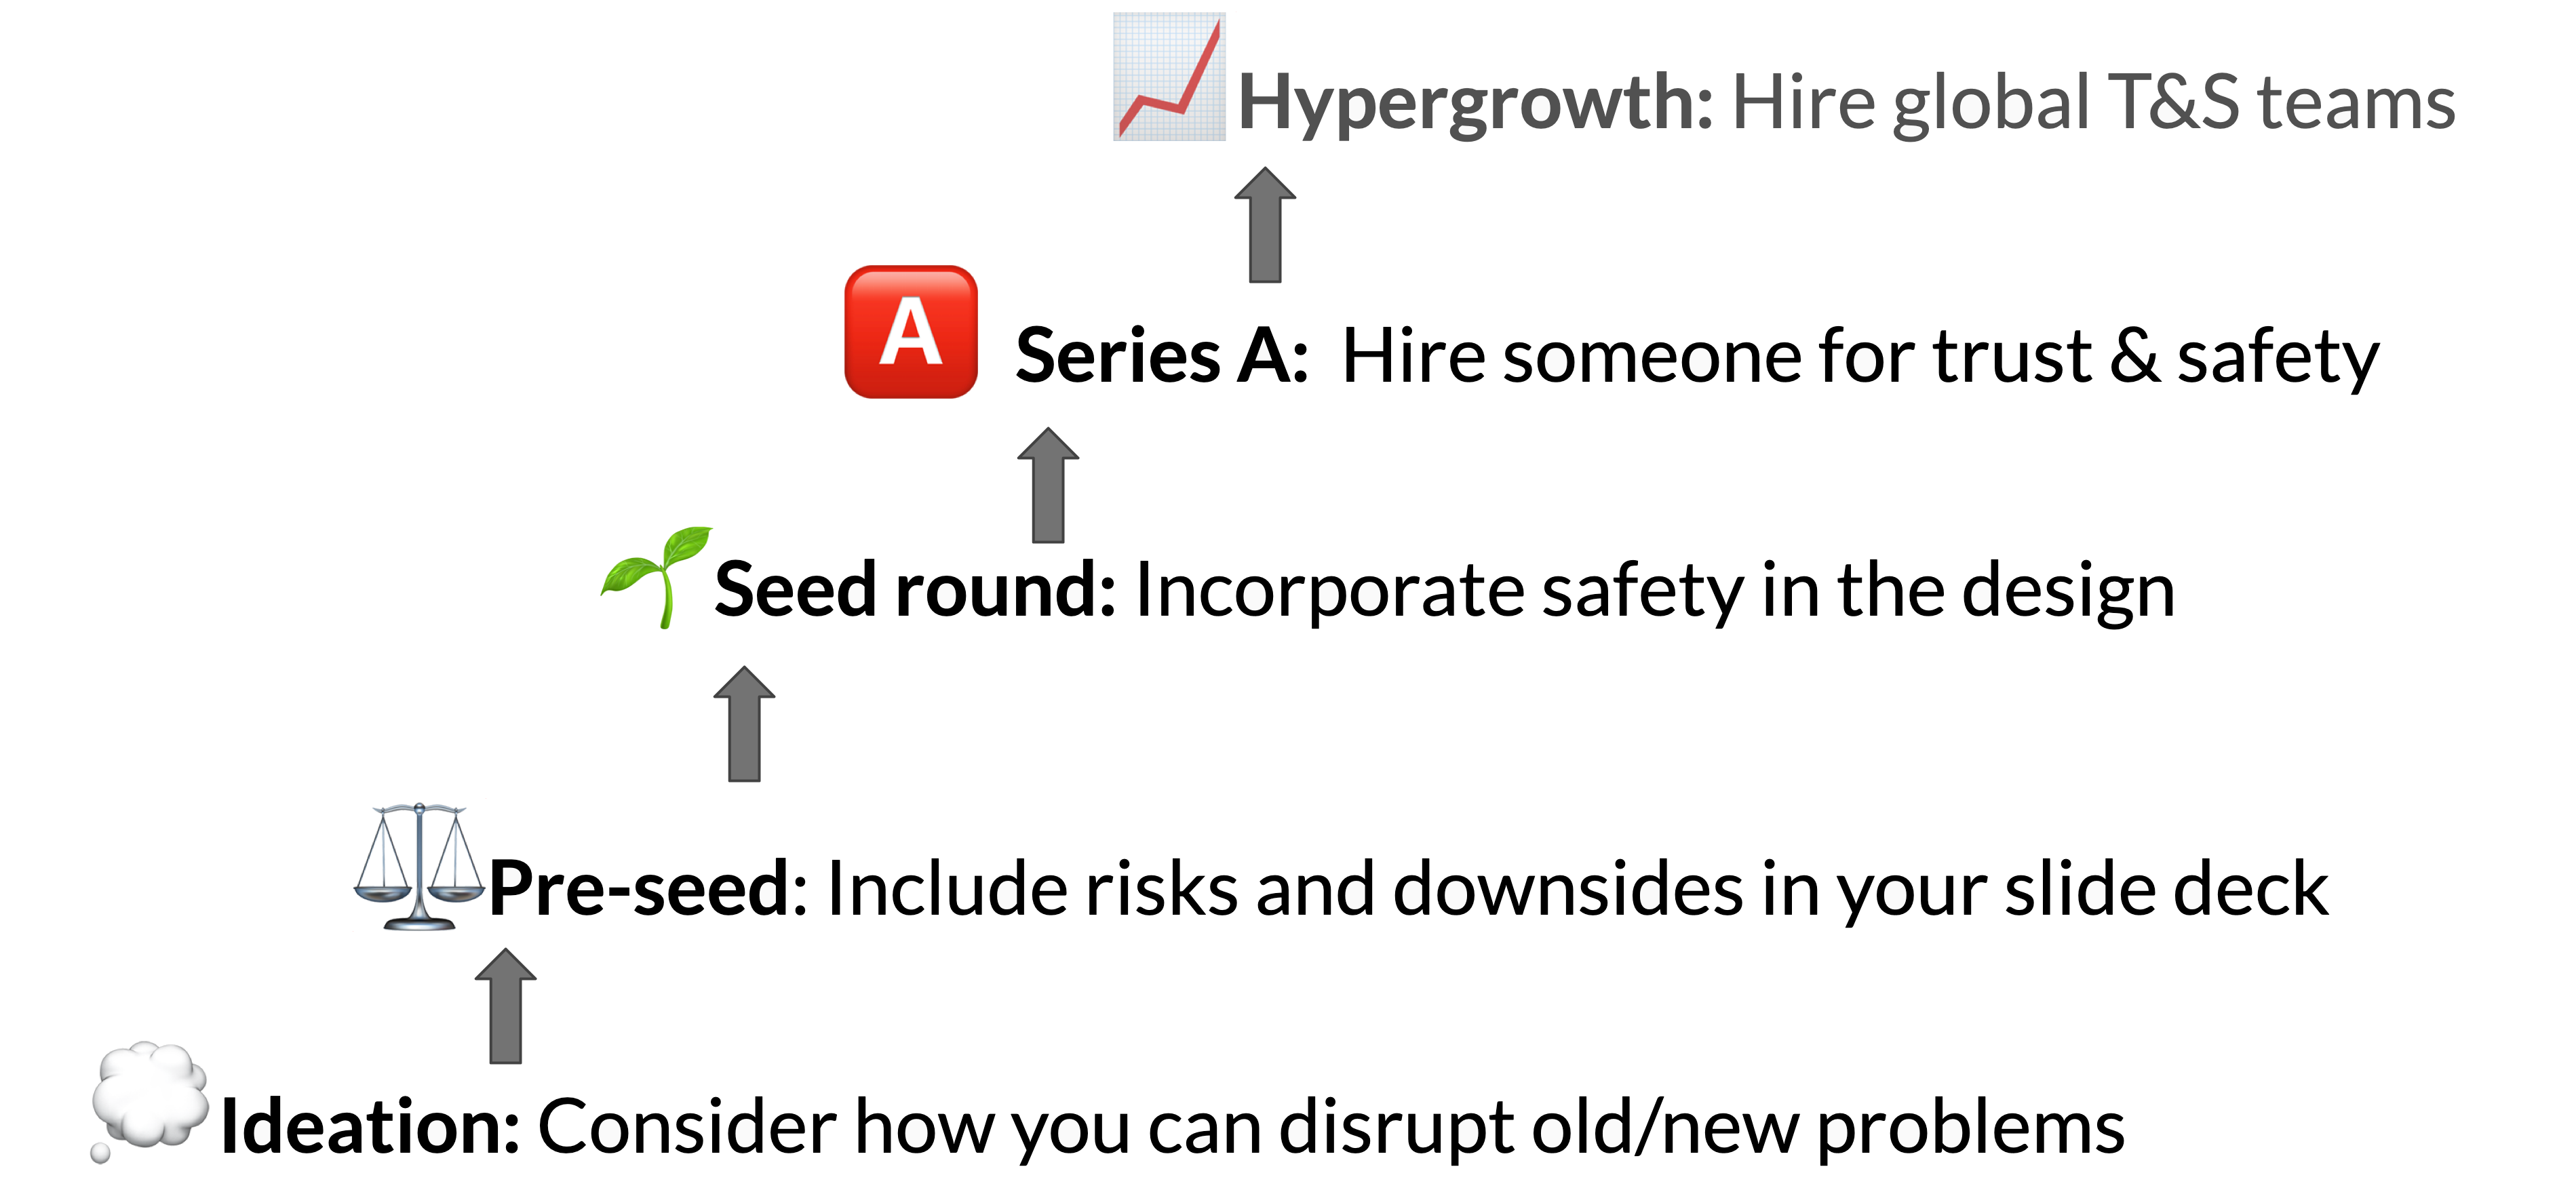
\includegraphics[width=\textwidth]{company-lifecycle}
\end{frame}

\end{document}